%--------------------------------------------------------------
%	Trabajo Especial de Grado
%	Autor: Pedro Luis Boll Lugo
%--------------------------------------------------------------

%--------------------------------------------------------------
%	ARCHIVO PRINCIPAL
%--------------------------------------------------------------

%	Tipo de documento
\documentclass[letterpaper,12pt]{report}

%	Lista de paquetes a utilizar
\usepackage[utf8]{inputenc}
\usepackage{graphicx}
\usepackage[spanish, mexico,es-tabla]{babel}
\usepackage{url}
\usepackage{cite}
\usepackage[right=3cm,left=3cm,top=2cm,bottom=2.2cm,headsep=0.5cm,footskip=0.5cm]{geometry}
\usepackage{fancyhdr}
\usepackage{emptypage}
\usepackage[nottoc,notlot,notlof]{tocbibind}
\usepackage[justification=centering]{caption}
\usepackage[table]{xcolor}
\usepackage{color}
\usepackage{colortbl}
\usepackage{multicol}
\usepackage{multirow}
\usepackage{booktabs}
\usepackage{tabularx}
\usepackage{array}
\usepackage{longtable}

%	Ubicación de las imágenes 
\graphicspath{ {Figuras/} }


% 	Aquí definimos el encabezado de las paginas 
\lhead[L]{}
\chead[]{}
\rhead[]{\thepage}
\renewcommand{\headrulewidth}{0.2pt}


% 	Aquí definimos el pie de pagina de las paginas
%\lfoot[]{}
%\cfoot[]{}
%\rfoot[]{Herramienta de Automatización, Monitoreo y Análisis de Componentes y Artefactos basados en el Internet de las Cosas}
%\renewcommand{\footrulewidth}{0.2pt}

% 	Aquí definimos el encabezado y pie de pagina de la pagina inicial de un capitulo.
\fancypagestyle{plain}{
%	Encabezado
\fancyhead[L]{\rightmark}
\fancyhead[C]{}
\fancyhead[R]{\thepage}
%	Pie de pagina
%\fancyfoot[L]{}
%\fancyfoot[C]{}
%\fancyfoot[R]{Herramienta de Automatización, Monitoreo y Análisis de Componentes y Artefactos basados en el Internet de las Cosas}
\renewcommand{\headrulewidth}{0.2pt}
%\renewcommand{\footrulewidth}{0.2pt}
}
\setlength{\headheight}{16pt}

%	Estilo de las paginas (Activa encabezados y pie de pagina)
\pagestyle{fancy}


%	Tipo de referencias
\bibliographystyle{unsrt}

%	Titulo del documento
\title{Trabajo Especial de Grado}
%	Autor del documento
\author{Pedro Luis Boll Lugo}

%***************** Estructura del documento *****************

\begin{document}
%	Portada
%	Estilo de la pagina vacío
\thispagestyle{empty}

%	Forma de la pagina y centrado
\begin{minipage}[c][0.01\textheight][t]{0.85\textwidth}
\begin{center}

%	Logo de la universidad
\includegraphics[scale=0.8]{./Figuras/ucv_logo.jpg}

\bigskip\bigskip\bigskip

{\centering \scshape \large
%	Universidad 
UNIVERSIDAD CENTRAL DE VENEZUELA \\
%	Facultad
FACULTAD DE CIENCIAS \\
%	Escuela
ESCUELA DE COMPUTACIÓN \\[38pt]}


\bigskip
{\scshape \LARGE 
%	Titulo del documento
Herramienta de Automatización, Monitoreo y Análisis de Componentes y Artefactos basados en el Internet de las Cosas 
\\[60pt]} 

\vspace{5mm}

{ \scshape \renewcommand\baselinestretch{1}\selectfont    
%	Nombre y Apellido
Pedro Luis Boll Lugo\\
%	Cédula de identidad
Cédula: 20.173.376 \\[30pt]

%Tutores:
Tutor:\\
Prof. Antonio Russoniello\\[30pt]

\vspace{10mm}

%	Fecha del documento
Caracas, Octubre 2023\\[60pt]
\vfill
}


\end{center}
\end{minipage}
%   Agradecimientos
%-----------------------------------------------------------------------------
%	Resumen
%-----------------------------------------------------------------------------
\chapter*{Agradecimientos}
\addcontentsline{toc}{chapter}{Agradecimientos}
\markboth{Agradecimientos}{Agradecimientos} 

.\\ 



\vspace{\fill} 
Palabras Claves:. 
% 	Resumen
%-----------------------------------------------------------------------------
%	Resumen
%-----------------------------------------------------------------------------
\chapter*{Resumen}
\addcontentsline{toc}{chapter}{Resumen}
\markboth{Resumen}{Resumen} 

Este es el espacio para el resumen .\\ 



\vspace{\fill} 
Palabras Claves: palabra clave 1, palabra clave 2, palabra clave 3.
\vspace{20px} 
%	Indice / Tabla de Contenidos
%--------------------------------------------------------------
%	Agregando las subsubsecciones a los indices
%--------------------------------------------------------------
\setcounter{secnumdepth}{4} 
\setcounter{tocdepth}{4} 

%--------------------------------------------------------------
%	Indice de contenidos
%--------------------------------------------------------------
\tableofcontents

%--------------------------------------------------------------
%	Indice de Figuras
%--------------------------------------------------------------
\newpage
\addcontentsline{toc}{chapter}{Lista de figuras}
\listoffigures

%--------------------------------------------------------------
%	Indice de Tablas
%--------------------------------------------------------------
\newpage
\addcontentsline{toc}{chapter}{Lista de tablas}
\listoftables



%	Introducción
%-----------------------------------------------------------------------------
%	 Marco Introductorio
%-----------------------------------------------------------------------------

\lhead[\thepage]{Marco Introductorio \thechapter. \rightmark}
\rhead[Marco Introductorio \thechapter. \leftmark]{\thepage}

%	Capitulo 1: Marco Introductorio
\chapter{Introducción}
\markboth{Introducción}{Introducción}
En general la adopción de nuevas tecnologías suele ocurrir de manera dispar. En algunas ocasiones la adopción es lenta y paulatina lo cual permite que pueda madurar en los diversos entornos en donde se implantan así como también permite crear formas ordenadas y planificadas de crecimiento de los elementos que se encuentran involucrados. Por otro lado también existen tecnologías que debido a su rápido crecimiento hacen que las personas y organizaciones deban adaptarse y ser flexibles en la manera en que se piensa se deben usar los avances, así como también la gama completa de oportunidades y debilidades que representa su uso.\\ 

Una de esas tecnologías que ha cambiado la manera en que los seres humanos actuamos es el computador personal. Con el acceso a una plataforma tan poderosa, la capacidad de poder automatizar elementos de la vida cotidiana y de procesos complejos en las industrias, se tiene la receta para ser una de las herramientas más importantes que haya creado el hombre. \\

Otra tecnología que ha cambiado al mundo es la capacidad de acceder y compartir información a través de una red. Su evolución a lo largo del tiempo a lo que ahora es el internet ha sido uno de los avances cruciales en la historia. No es una tecnología reciente, pero se ha masificado y democratizado su acceso de tal forma que es un aspecto omnipresente para mas de la mitad de la población mundial. Las diversas plataformas que se apoyan en la "red de redes" nos han ayudado a masificar la adopción de otro conjunto enorme de otras tecnologías, pues su flexibilidad y la madurez de los procesos que involucran la capacidad de conexión es catalizador de oportunidades para resolver problemas.\\

Si juntamos los aspectos de computo y conectividad vemos que de manera disruptiva actualmente se tiene la oportunidad de mejorar y automatizar muchos de los procesos que antes por costo, logística o complejidad eran difíciles de llevar a cabo. El crecimiento en la información y en masificación de artefactos y elementos que obtienen datos de su entorno proveen a los involucrados de una nueva visión del funcionamiento de las cosas que no era posible. Es esta revolución de la información la llamamos ``internet de las cosas" (o IoT por sus siglas en ingles) y es una tendencia en la tecnología en pleno crecimiento y que seguirá creciendo de manera activa en los años por venir.\\ 

Sin embargo como en casi todo nuevo avance en la tecnología, no ha venido sin presentar retos y dificultades propias. El gran volumen de información generado de manera automatizada, el control y monitoreo de dispositivos y artefactos a lo largo y ancho de complejos sistemas y y nuevos flujos automáticos donde antes no eran posibles de realizar hacen cada vez mas difícil el poder tener un panorama claro de las operaciones de estos sistemas por lo que se requieren de infraestructuras, plataformas y desarrollos nuevos para poder mejorar los aspectos de adopción mas ordenada de una forma tan nueva de hacer las cosas. Es así como nace la propuesta de comenzar a realizar la integración de tecnologías probadas que juntas puedan dar un mejor panorama en la observación y control de elementos de las operaciones y acciones que llevamos a cabo de manera automatizada en nuestro día a día.\\

En el siguiente trabajo de investigación se presenta una propuesta de un software que sea capaz de brindar la capacidad de mostrar datos en tiempo real e histórica provenientes de sensores y actuadores de dispositivos basados en el internet de las cosas, así como también la capacidad de crear flujos de automatización y control de los mismos, de forma que sea una plataforma centralizada para la gestión de los dispositivos IoT dentro de un ambiente en específico.\\

En el capitulo dos presentamos de una manera detallada el problema de investigación, los antecedentes y motivaciones que llevan a examinar este problema desde el punto de vista investigativo, así como cuales son los principios que justifican indagarlo. Con ese conocimiento podemos presentar una solución en donde se tiene el alcance del proyecto, así como también de plantean los objetivos generales y específicos con los que abordaran del punto de vista metodológico.\\

En los capítulos tres y cuatro se presentan los conceptos teóricos requeridos para abarcar los procesos mencionados previamente, en un primer momento tomando el concepto de internet de las cosas de manera clara y las ventajas y desventajas que ha tenido la adopción de este tipo de tecnologías en la sociedad y luego presentando un panorama sobre las herramientas de visualización y de control existentes y como el enfoque adecuado puede ayudar a cerrar la brecha entre los datos que se van generando y las gestión de dispositivos que son cada vez mas omnipresentes como complejos.\\

Para los capítulos cinco, seis y siete presentamos el marco metodológico utilizado para diseñar, crear, probar y validar el funcionamiento integral de los componentes desarrollados con el fin de poder cumplir con los objetivos planteados, incluyendo los posibles escenarios donde este proyecto puede dar un valor agregado a las estructuras existentes. \\
 
Por último, los capítulos ocho y nueve nos dan la presentación de los resultados finales tras el desarrollo, entendiendo las circunstancias con la que se desarrollo el problema y sugiriendo una serie de trabajos futuros pueden llevarse a cabo a partir de esta base. Ademas se establecen las conclusiones finales a las que se llegan marcando la tesis mencionada después de todo el trabajo investigativo realizado. \\

%	Capitulo uno
%-----------------------------------------------------------------------------
%	 Problema de Investigación
%-----------------------------------------------------------------------------

\lhead[\thepage]{Problema de Investigación \thechapter. \rightmark}
\rhead[Problema de Investigación \thechapter. \leftmark]{\thepage}

%	Capitulo 4: Problema de Investigación
\chapter{Problema de Investigación}
\markboth{Problema de Investigación}{Problema de Investigación}

%	Sección uno: Planteamiento del Problema
\section{Planteamiento del Problema}
\lhead[\thepage]{\thesection. Planteamiento del Problema}
Cada día es mas común el poder observar dispositivos y artefactos que consideramos normales, adquirir capacidades de conexión, de captura de datos y capaces de ejercer acciones sobre el ambiente. A estos dispositivos son parte de un boom tecnológico al cual se le llama Internet de las Cosas y su importancia radica en que cambiaran la manera con la que interactuamos con los ambientes en donde hacemos vida, como nuestros, trabajos, hogares y ciudades.\\

El Internet de las Cosas abre la puerta a un grupo importante de innovaciones a todo nivel y un lugar que se beneficiará de esto serán los hogares.  La idea de tener artefactos, dispositivos y electrodomésticos que sean cada vez mas autónomos no es nueva, pero la domótica ya esta teniendo una evolución en cuanto a la manera en que estos no solo adquieren capacidad de comunicarse con otros sistemas sino como interactuamos con nuestros hogares, con el fin de automatizar aquellas labores tediosas y difíciles, de proveer de mayores niveles de seguridad a nuestros bienes y a nuestros seres queridos y finalmente interactuar de maneras ineditas.\\

Es así como los procesos del hogar se van automatizando gracias a estos artefactos inteligentes y que son capaces de medir variables de interés, como el consumo de los recursos del hogar, alertas de sensores de vigilancia o aquellos datos generados por experiencias de usuario personalizadas. En la actualidad existen sistemas y plataformas (tanto libres como propietarias) que permiten conocer el estado actual de las métricas obtenidas de los dispositivos y controlarlos usando recetas de comportamiento preestablecidas y programables.\\ 

Una cualidad importante de estos sistemas es que los dispositivos y artefactos conectados aportan una gran cantidad de datos que pueden ser útiles para la toma de decisiones tanto automatizada como no automatizada. Sin embargo, un reto que debe afrontarse es que ante la creciente cantidad de dispositivos IoT que se suman a los sistemas domóticos se necesitan sistemas que sean capaces no solamente de mostrar una instantánea del estado actual de los sensores, actuadores y dispositivos en general en el hogar, sino el poder almacenar y procesar todos los datos (muchos de ellos semi-estructurados o no estructurados) que se producen de manera continua, con el fin de encontrar información que pueda ser utilizada tanto para mejorar los proceso en los que se busca determinar patrones de consumo, puntos de falla y optimizar el manejo y control de los aspectos automatizables del hogar.\\

Dadas las características y complejidad que implica este problema, surgen las preguntas de ¿cual es la mejor arquitectura para un sistema domótico que aproveche todos los datos que se generan?, ¿requieren estos datos algún tratamiento especial para su almacenamiento?, ¿qué información es posible obtener de los datos recabados de los dispositivos y sus procesos a través de un sistema domótico y que conocimiento nos pueden dejar?, y finalmente ¿es posible que al tener ese conocimiento se pueda realizar una toma de decisiones automatizadas que tengan en cuenta inteligentemente las condiciones actuales del ambiente, así como también los gustos de las personas, de forma de ajustar el funcionamiento de los dispositivos?

\subsection{Justificación}
Los datos generados por el uso y consumo de recursos, por las estadísticas y operaciones de sistemas domóticos en la actualidad tiene un carácter comercial poco explorado. Muchos de los recursos utilizados en los hogares no cuentan con inspección o solo se obtienen métricas de forma global a través de la facturación de los proveedores de los servicios. Esta tendencia está cambiando poco a poco pero abre la oportunidad de ofrecer tanto en hogares construidos o como en los diseños de los nuevos hogares inteligentes, de forma que puedan aportar características de eficiencia energética, de consumo de recursos vitales y su reposición sustentable y de mayores niveles de seguridad y confort para los habitantes.\\

La respuesta a diversas preguntas planteadas en la investigación pasa por la creación una herramienta analítica diseñada para tratar con grandes volúmenes de datos, que sea software libre y capaz de integrarse con soluciones existentes utilizadas para monitorear y controlar dispositivos IoT, con la cual se puedan obtener modelos que revelen patrones de consumo y uso sobre uno o mas procesos automatizados o automatizables en el hogar.

\subsection{Alcance}
Como se explico en la sección automatización de hogar existen cuatro posible campos de acción automatizables del hogar que son la administración y monitoreo de recursos (energía, luz, HVACS, agua, desperdicios, etc), la seguridad del hogar, la accesibilidad y el uso de sistemas para el entretenimiento y confort de las personas. Con esto en mente se plantea la creación de una herramienta de análisis de datos al cual se pueda integrar con  un sistema de automatización de hogares, que controle y registre datos de uno o mas dispositivos cuyos sensores sobre uno los campos de acción de automatización de hogar, que ademas sea fácil de escalar y con un costo bajo de implementación. 

\subsection{Objetivos}
\subsubsection{Objetivos Generales}
El objetivo de esta investigación es el poder determinar la mejor estrategia para afrontar el desarrollo de un sistema de domótico inteligente y adaptado al Internet de las Cosas, con la capacidad de analizar los datos históricos y actuales del hogar para optimizar los procesos automatizados, haciendo uso de técnicas de Big data.
\subsubsection{Objetivos Específicos}
Para alcanzar el objetivo general estipulado se plantean los siguientes objetivos específicos:
\begin{itemize}
\item Utilizar la metodología Scrum durante el diseño y creación de las herramientas durante todo el proceso. 
\item Establecer la arquitectura adecuada para dar soporte a un sistema domótico y el software de análisis de los datos de dispositivos IoT.
\item Seleccionar el software de gestión domótico adecuado y que permita la integración de la herramienta de análisis a crear.
\item Seleccionar y utilizar herramientas diseñadas para trabajar con grandes volúmenes de datos y construir un pequeño cluster en el cual desplegarlas.
\item Construir prototipos funcionales de uno o mas dispositivos IoT para la captura de datos de las variables sobre los procesos que están monitoreando y automatizando.
\item Realizar la captura de datos y la construcción de modelos bajo metodología KDD y Fundamental Methodology for Data Science para el análisis de los mismos y generar conocimiento útil para los usuarios.
\item Establecer comportamientos dinámicos en base al conocimiento obtenido en los prototipos funcionales.
\item Utilizar herramientas de visualización de datos adecuadas para informar los resultados obtenidos y realizar sugerencias.
\end{itemize}

%	Capitulo dos
%-----------------------------------------------------------------------------
%	 Internet de las Cosas
%-----------------------------------------------------------------------------

\lhead[\thepage]{Internet de las Cosas \thechapter. \rightmark}
\rhead[Internet de las Cosas \thechapter. \leftmark]{\thepage}

%	Capitulo N: Internet de las Cosas
\chapter{Internet de las Cosas}
\markboth{Internet de las Cosas}{Internet de las Cosas}
\section{Definición}
El ``Internet de las Cosas", también conocido como IoT por sus siglas en inglés es el término utilizado para designar al conjunto de artefactos y dispositivos que poseen la capacidad de conectarse entre ellos o a otras redes como el internet de forma que pueden transmitir y recibir datos e información. De manera formal no existe una definición estandarizada sobre el concepto de IoT, pues dependiendo de la organización puede considerarse el concepto desde el punto de vista desde el cual se observe el concepto, sea desde la perspectiva de las redes, desde el punto de vista de los dispositivos o bien desde el punto de vista de los sistemas automatizados.\\

La primera aparición del término fue realizada en la conferencia ``Congressional Black Caucus Foundation 15th Annual Legislative Weekend'' en Washington, D. C. en septiembre del año 1985 por parte de Peter Lewis \cite{IoTTrueHistory} en donde define que ``El Internet de las cosas, o IoT, es la integración de personas, procesos y tecnología con dispositivos y sensores conectables para permitir el monitoreo, estado, manipulación y evaluación remota de las tendencias de dichos dispositivos''\cite{IoTFirstDef}.\\

Sin embargo este concepto fue olvidado hasta el año 1999 cuando Kevin Ashton independientemente lo utilizó ilustrar el poder de conectar Etiquetas de Identificación por Radio Frecuencia (RFID) usadas en las cadenas de suministro corporativas a Internet para contar y rastrear mercancías sin la necesidad de intervención humana\cite{iotInternetSociety}.\\

Para fines prácticos, durante esta investigación se toma el concepto de original de Peter Lewis, al ser una propuesta genérica e independiente del aspecto funcional examinado. Sin embargo es importante recalcar el hecho que las Las diversas definiciones de IoT no necesariamente están en desacuerdo, sino que enfatizan diferentes aspectos de las tecnologías aplicadas sobre los dispositivos IoT desde diferentes puntos focales y casos de uso. \cite{iotInternetSociety}

\vspace{50px}

\section{Modelos de Comunicación}
Desde el punto de vista teórico, los dispositivos IoT pueden interconectarse de varias formas. Estos siguen el marco de desarrollo planteado por el estandar RFC-7452\cite{rfc7452} en el que se plantean 4 modelos de comunicación con características propias. Esos modelos son:

\subsection{Comunicación Dispositivo a Dispositivo}
Este modelo de comunicación es el mas simple de todos los paradigmas y consiste básicamente en poder conectar directamente los dispositivos independientemente del medio usado Los dispositivos se comunican usando alguno de los protocolos y estándares disponibles que sean capaces de comprender. En el ámbito del IoT esta comunicación se realiza de manera inalambrica y donde los datos o instrucciones suelen ser bastante pequeños o poco frecuentes (figura \ref{fig:d2d}). En grandes cantidades estaríamos en presencia de un modelo netamente distribuido.
\begin{figure}[htb]
\centering
\includegraphics[scale=0.4]{./Figuras/d2d.png}
\caption{Modelo dispositivo a dispositivo}
\label{fig:d2d}
\end{figure}

  
\subsection{Comunicación Dispositivo a la Nube}
En el modelo de comunicación dispositivo a la nube, la conexión del dispositivo se conecta directamente a una nube (propia o federada) usando un proveedor de servicio (figura \ref{fig:d2n}). Este enfoque frecuentemente se aprovecha de los mecanismos de comunicación como redes celulares o la infraestructura de procesamiento de una  organización de manera directa para establecer la conexión entre el dispositivo y el servicio en la nube.
\begin{figure}[htb]
\centering
\includegraphics[scale=0.4]{./Figuras/d2n.png}
\caption{Modelo dispositivo a la nube}
\label{fig:d2n}
\end{figure}

\subsection{Comunicación Dispositivo a Puerta de Enlace}
El modelo de comunicación dispositivo a puerta de enlace establece una dispositivo o capa intermedia que concentre todas las comunicaciones (hub o broker) entre los dispositivos y de allí de ser necesario a otros fragmentos de la red o a internet (figura \ref{fig:d2g}). La ventaja de este enfoque es la capacidad de operar de manera centralizada parte de las comunicaciones de los dispositivos. Muchos protocolos están basados en el principio del paradigma de cliente-servidor por lo que este se adapta de manera natural al modelo.
\begin{figure}[htb]
\centering
\includegraphics[scale=0.4]{./Figuras/d2g.png}
\caption{Modelo dispositivo a puerta de enlace}
\label{fig:d2g}
\end{figure}

\subsection{Comunicación Dispositivo a Intercambio de Datos en Back-end}
Este modelo es una forma automatizada de conexiones, en donde el dispositivo envía los datos a una o más APIs para de manera transparente, haciendo que este pueda intercambiar la información entre servicios que no necesariamente están estructurados o que pertenecen a un tercero (figura \ref{fig:d2b}). Particularmente este modelo es útil cuando se requiere que la información sea fácilmente accesible a través de múltiples plataformas o sistemas independientes.
\begin{figure}[htb]
\centering
\includegraphics[scale=0.4]{./Figuras/d2b.png}
\caption{Modelo dispositivo a intercambio de datos en back-end}
\label{fig:d2b}
\end{figure}


\section{Aplicaciones del Internet de las Cosas}
hue
\subsection{Hogares}
hue
\subsection{Industrias}
hue
\subsection{Transporte y Logistica}
hue
\subsection{Comercio}
hue
\subsection{Tecnologías Vestibles}
hue
\subsection{Medicina y Salud}
hue
\subsection{Ciudades Inteligentes}
hue

\section{Interoperatividad entre Infraestructuras y Dispositivos}
hue
\subsection{Ecosistemas}
hue
\subsection{Restricciones}
hue
\subsection{Riesgos}
hue
\subsection{Sistemas Heredados}
hue
\subsection{Configuración de dispositivos}
hue

\section{Protocolos y Estándares Utilizados}
hue
\subsection{Protocolos}
hue
\subsubsection{HTTP}
hue
\subsubsection{MQTT}
hue
\subsubsection{IPv4 e IPv6}
hue
\subsection{Estándares}
hue
\subsubsection{Bluetooth}
hue
\subsubsection{Redes Celulares}
hue
\subsubsection{NFC}
hue
\subsubsection{Wifi}
hue
\subsubsection{Zigbee}
hue
\subsubsection{Z-Wave}
hue

\section{Seguridad}
hue.

%	Capitulo tres
%-----------------------------------------------------------------------------
%	 Herramientas de Monitoreo, Visualización y Control
%-----------------------------------------------------------------------------

\lhead[\thepage]{Herramientas de Monitoreo, Visualización y Control \thechapter. \rightmark}
\rhead[Herramientas de Monitoreo, Visualización y Control \thechapter. \leftmark]{\thepage}

%	Capitulo 4: Herramientas de Monitoreo, Visualización y Control
\chapter{Herramientas de Monitoreo, Visualización y Control}
\markboth{Herramientas de Visualización y Control}{Herramientas de Monitoreo, Visualización y Control}
hue

\section{Herramientas de Monitoreo}
hue

\section{Herramientas de Visualización}
hue

\section{Herramientas de Control}
hue

%	Capitulo cuatro
%-----------------------------------------------------------------------------
%	 Placas Programables
%-----------------------------------------------------------------------------

\lhead[\thepage]{Placas Programables \thechapter. \rightmark}
\rhead[Placas Programables \thechapter. \leftmark]{\thepage}

%	Capitulo 5: Placas Programables
\chapter{Placas Programables}
\markboth{Placas Programables}{Placas Programables}

%	Sección uno: Definición
\section{Definición}
\lhead[\thepage]{\thesection. Definición}
Las placas programables, también llamadas placas de programación o desarrollo son dispositivos básicos que cuentan con un microcontrolador programable con el cual se pueden ejecutar diferentes instrucciones. En muchos escenarios estamos en presencia de una computadora de recursos muy reducidos (conocidos como Single Board Computer o SBC por sus siglas en inglés), pues siguen al pie de la letra con la arquitectura del computador de John von Nuemann\cite{arquitecturaComputador}.\\ 

Estas computadoras de una sola placa se hicieron como sistemas de demostración o desarrollo, para sistemas educativos o para su uso como controladores integrados de computación los que las hace especialmente útiles para poder crear prototipos funcionales de dispositivos de toda clase, desde robots hasta dispositivos de Internet de las cosas. Para poder crear las rutinas se hacen uso de lenguajes de programación que establecen el control directo contra la microprocesador o incluso contra los sensores y actuadores que puedan estar conectados al dispositivo.\\

Algunas placas incluso poseen la capacidad de soportar un sistema operativo completo los cuales los hacen inmensamente flexibles a la hora de realizar tareas, de agregar nuevos sensores o controlar otros dispositivos a través de esa placa. Existen gran cantidad de modelos distintos en el mercado. Sin embargo en este trabajo de investigación nos centraremos en dos tipos de placas en específico:

%	Sección dos: Placas Arduino
\section{Placas Arduino}
\lhead[\thepage]{\thesection. Placas Arduino}
Arduino (Genuino a nivel internacional es una plataforma electrónica en hardware y software libres, fáciles de usar. Está pensado para cualquier persona que haga proyectos interactivos.\cite{ArduinoOfficial}(figura \ref{fig:arduino_logo}) Las placas Arduino tiene la capacidad  detectar el ambiente recibiendo entradas de variedad de sensores, y afecta su entorno controlando luces, motores y otros actuadores. La lógica de micro controlador Arduino deberá hacerse escribiendo código en el lenguaje de programación Arduino (basado en C++) y utilizando el entorno de desarrollo de Arduino.\\

\begin{figure}[htb]
\centering
\includegraphics[scale=0.35]{./Figuras/arduino_logo.png}
\caption{Logo del proyecto Arduino}
\label{fig:arduino_logo}
\vspace*{-10pt}
\end{figure}

Arduino nació en el Ivrea Interaction Design Institute como una herramienta fácil para el prototipado rápido, dirigido a estudiantes sin formación en electrónica y programación. Tan pronto como llegó a una comunidad más amplia, la junta de Arduino comenzó a cambiar para adaptarse a las nuevas necesidades y desafíos, diferenciando su oferta de simples placas de 8 bits a productos para aplicaciones IoT, portátiles, impresión 3D y dispositivos embebidos. Todas las placas de Arduino son totalmente de hardware libre, lo que permite a los usuarios construirlas independientemente y eventualmente adaptarlas a sus necesidades particulares. El software, también es de código abierto y está creciendo a través de las contribuciones de los usuarios de todo el mundo.\\

Las placas Arduino están disponibles de dos formas: ensambladas o en forma de kits ``Hágalo tú mismo''. Los esquemas de diseño del hardware están disponibles bajo licencia Libre, con lo que se permite que cualquier persona pueda crear su propia placa Arduino sin necesidad de comprar una prefabricada. La primera placa Arduino fue introducida en 2005 llamada Arduino Uno \ref{fig:arduinouno}), ofrecida a un bajo costo y facilidad de uso para novatos y profesionales. Se buscaba desarrollar proyectos interactivos con su entorno mediante el uso de actuadores y sensores. A partir de octubre de 2012, se incorporaron nuevos modelos de placas de desarrollo que usan micro controladores Cortex M3, ARM de 32 bits, que coexisten con los originales modelos que integran micro controladores AVR de 8 bits.\\

En la actualidad, existen 29 distintas placas de micro controladores, 7 módulos complementarios, 15 Shields (placas de expansión), con lo cual se posee un ecosistema rico de diversos micro controladores para cada tarea o cada ambiente de desarrollo. 

\begin{figure}[htb]
\centering
\includegraphics[scale=0.7]{./Figuras/arduino_uno.jpeg}
\caption{Arduino Uno R3}
\label{fig:arduinouno}
\vspace*{-10pt}
\end{figure}

%	Sección tres: Placas Raspberry Pi
\section{Placas Raspberry Pi}
\lhead[\thepage]{\thesection. Placas Raspberry Pi}
Raspberry Pi es una marca (figura \ref{fig:raspi_logo}) de micro computadores de hardware libre, que comenzó como proyecto para llevar a la educación  de escolares ingleses conceptos de la computación, de la programación y de la electrónica, y que luego la comunidad Maker y algunas compañías adoptaron, pues vieron el potencial para crear dispositivos, sensores, actuadores, robots entre otros y para poder llevar a cabo prototipos funcionales de dispositivos y de productos muy rápidamente. El relativo bajo costo (que va desde \$10 por la placa mas sencilla hasta \$80 por el modelo más avanzado) y facilidad de uso, han facilitado la adopción de este micro computador por personas en todo el mundo para toda clase de proyectos amateurs y profesionales.

\begin{figure}[htb]
\centering
\includegraphics[scale=0.65]{./Figuras/raspi_logo.png}
\caption{Logo de la marca Raspberry Pi}
\label{fig:raspi_logo}
\vspace*{-10pt}
\end{figure}

Este es un proyecto llevado a cabo con la Raspberry Pi Foundation\cite{RaspberryPi} desde el año 2012 ofreciendo hasta el día de hoy siete modelos distintos de placas, con procesadores ARM, memoria RAM que va desde los 256MB hasta 1GB y cuya memoria es de carácter externo usando tarjetas MicroSD en la mayoría de los modelos y cuyo consumo no es mayor al de 2,5 amperios. Los modelos son:
\begin{itemize}
\item Raspberry Pi Modelo A: Fue el primer modelo de Raspberry Pi en salir al mercado, en el año 2012. Basado en un SoC Broadcom BCM28235, cuyo procesador es un ARM11 32 bits a 700MHz, Gráficas Broadcom VideoCore IV, con 256MB de memoria RAM, un puerto USB, una salida HDMI, un conector RCA, una entrada CSI para un modulo de cámara, y sin características de conectividad alguna por defecto. Para el almacenamiento se usan tarjetas SD. 
\item Raspberry Pi Modelo B/B+: También del año 2012, es una variante del Modelo A, trajo consigo diversas mejoras, como la inclusión del doble de memoria RAM, pasando de 256MB a 512MB. Trajo consigo un puerto USB más y un conector Ethernet (RJ-45) Se mantuvo tanto su tamaño como su coste. No hubo variaciones en el procesador ni en la gráfica. Tiempo después se lanzo el Modelo B+, que incluyó 4 puertos USB y pasó de usar una SD a una MicroSD.
\item Raspberry Pi 2 Modelo B: Lanzada en 2014 es el primer modelo que no incluye el mismo procesador usado en los tres anteriores: se sustituye por uno de la misma marca, pero de modelo BCM2836 con lo cual pasa de ser de un núcleo a cuatro, y de 700MHz a 900MHz, no obstante emplea la misma gráfica, la VideoCore IV. Dobla la cantidad de memoria RAM, pasando de 512MB a 1GB de memoria (también compartida con la gráfica). También incluye 40 pines GPIO, y mantiene los cuatro puertos USB. Suprime la conexión RCA.
\item Raspberry Pi 3 Modelo B: Sale al mercado en el año 2016, renovando procesador, una vez más de la compañía Broadcom, siendo un procesador de cuatro núcleos al igual que el modelo anterior, pero pasa de 900MHz a 1.20GHz,  manteniendo la RAM en 1GB. Su mayor novedad fue la inclusión de WiFi y Bluetooth (4.1 Low Energy) sin necesidad de adaptadores.
\item Raspberry Pi Zero: Fue el primer modelo miniaturizado de las Raspberry Pi, teniendo un tamaño un poco mayor a un Pen Drive. Lanzado en 2015 con un coste de 5 dólares, es una 40\% más potente que el primer modelo de Raspberry. Tiene un CPU Broadcom BCM2835, que funciona a 1GHz con dos núcleos. Posee 512MB de RAM, y comparte la gráfica VideoCore IV. Debido a su tamaño sustituye el puerto HDMI por MiniHDMI, manteniendo así las prestaciones. Tampoco usa USB estándar, sino que tiene dos MicroUSB, uno de alimentación y otro de datos. Posee salida RCA, pero en vez de por clavija son solo dos conectores integrados en la placa. Usa MicroSD como sistema de almacenamiento.(figura \ref{fig:rpizero})

\begin{figure}[htb]
\centering
\includegraphics[scale=0.25]{./Figuras/rpizero.png}
\caption{Raspberry Pi 4 modelo B}
\label{fig:rpizero}
\vspace*{-10pt}
\end{figure}

\item Raspberry Pi Zero W: Es la sucesora de la Raspberry Pi Zero. la W es por Wireless, ya que la única novedad de esta placa con respecto a su antecesora es la inclusión de WiFi y Bluetooth, por lo que su precio ascendió a 11 dólares.
\item Raspberry Pi 3 Modelo B+: Del mismo modo que para el Raspberry Pi Modelo B, esta es una actualización en términos de rendimiento sobre la Raspeberry Pi 3 Modelo B. Pasa a ser un poco más rápida que su antecesora y ofrece la capacidad de conectarse a Wifi doble banda. Incorpora Bluetooth 4.2 y la velocidad de su puerto ethernet pasa de 100 Mbits/seg a 300 Mbits/seg.
\item Raspberry Pi 3 Modelo A:  Los modelos A+ presentan menores prestaciones a un menor precio. Cuenta con 512 MB de RAM (compartidos con la GPU VideoCore IV), un solo puerto USB y sin puerto de conexión de red ethernet.
\item Raspberry Pi 4 modelo B: Esta versión viene a sustituir a la versiones 3 y cambia los puertos HDMI de tamaño completo por dos puertos microHDMI. Cuenta con la capacidad de manejar una pantalla a 4K a 60 Hz, o dos pantallas 4K a 30 Hz. Se ha incluido por primera vez USB 3.0, y el puerto Ethernet ya no está limitado a 300 Mbps. Tiene un procesador Broadcom nuevo. Es la primera serie que posee 3 variantes disponibles en los que cambia la cantidad de memoria RAM de 2GB, 4GB, y de 8GB (figura \ref{fig:rpi4}).

\begin{figure}[htb]
\centering
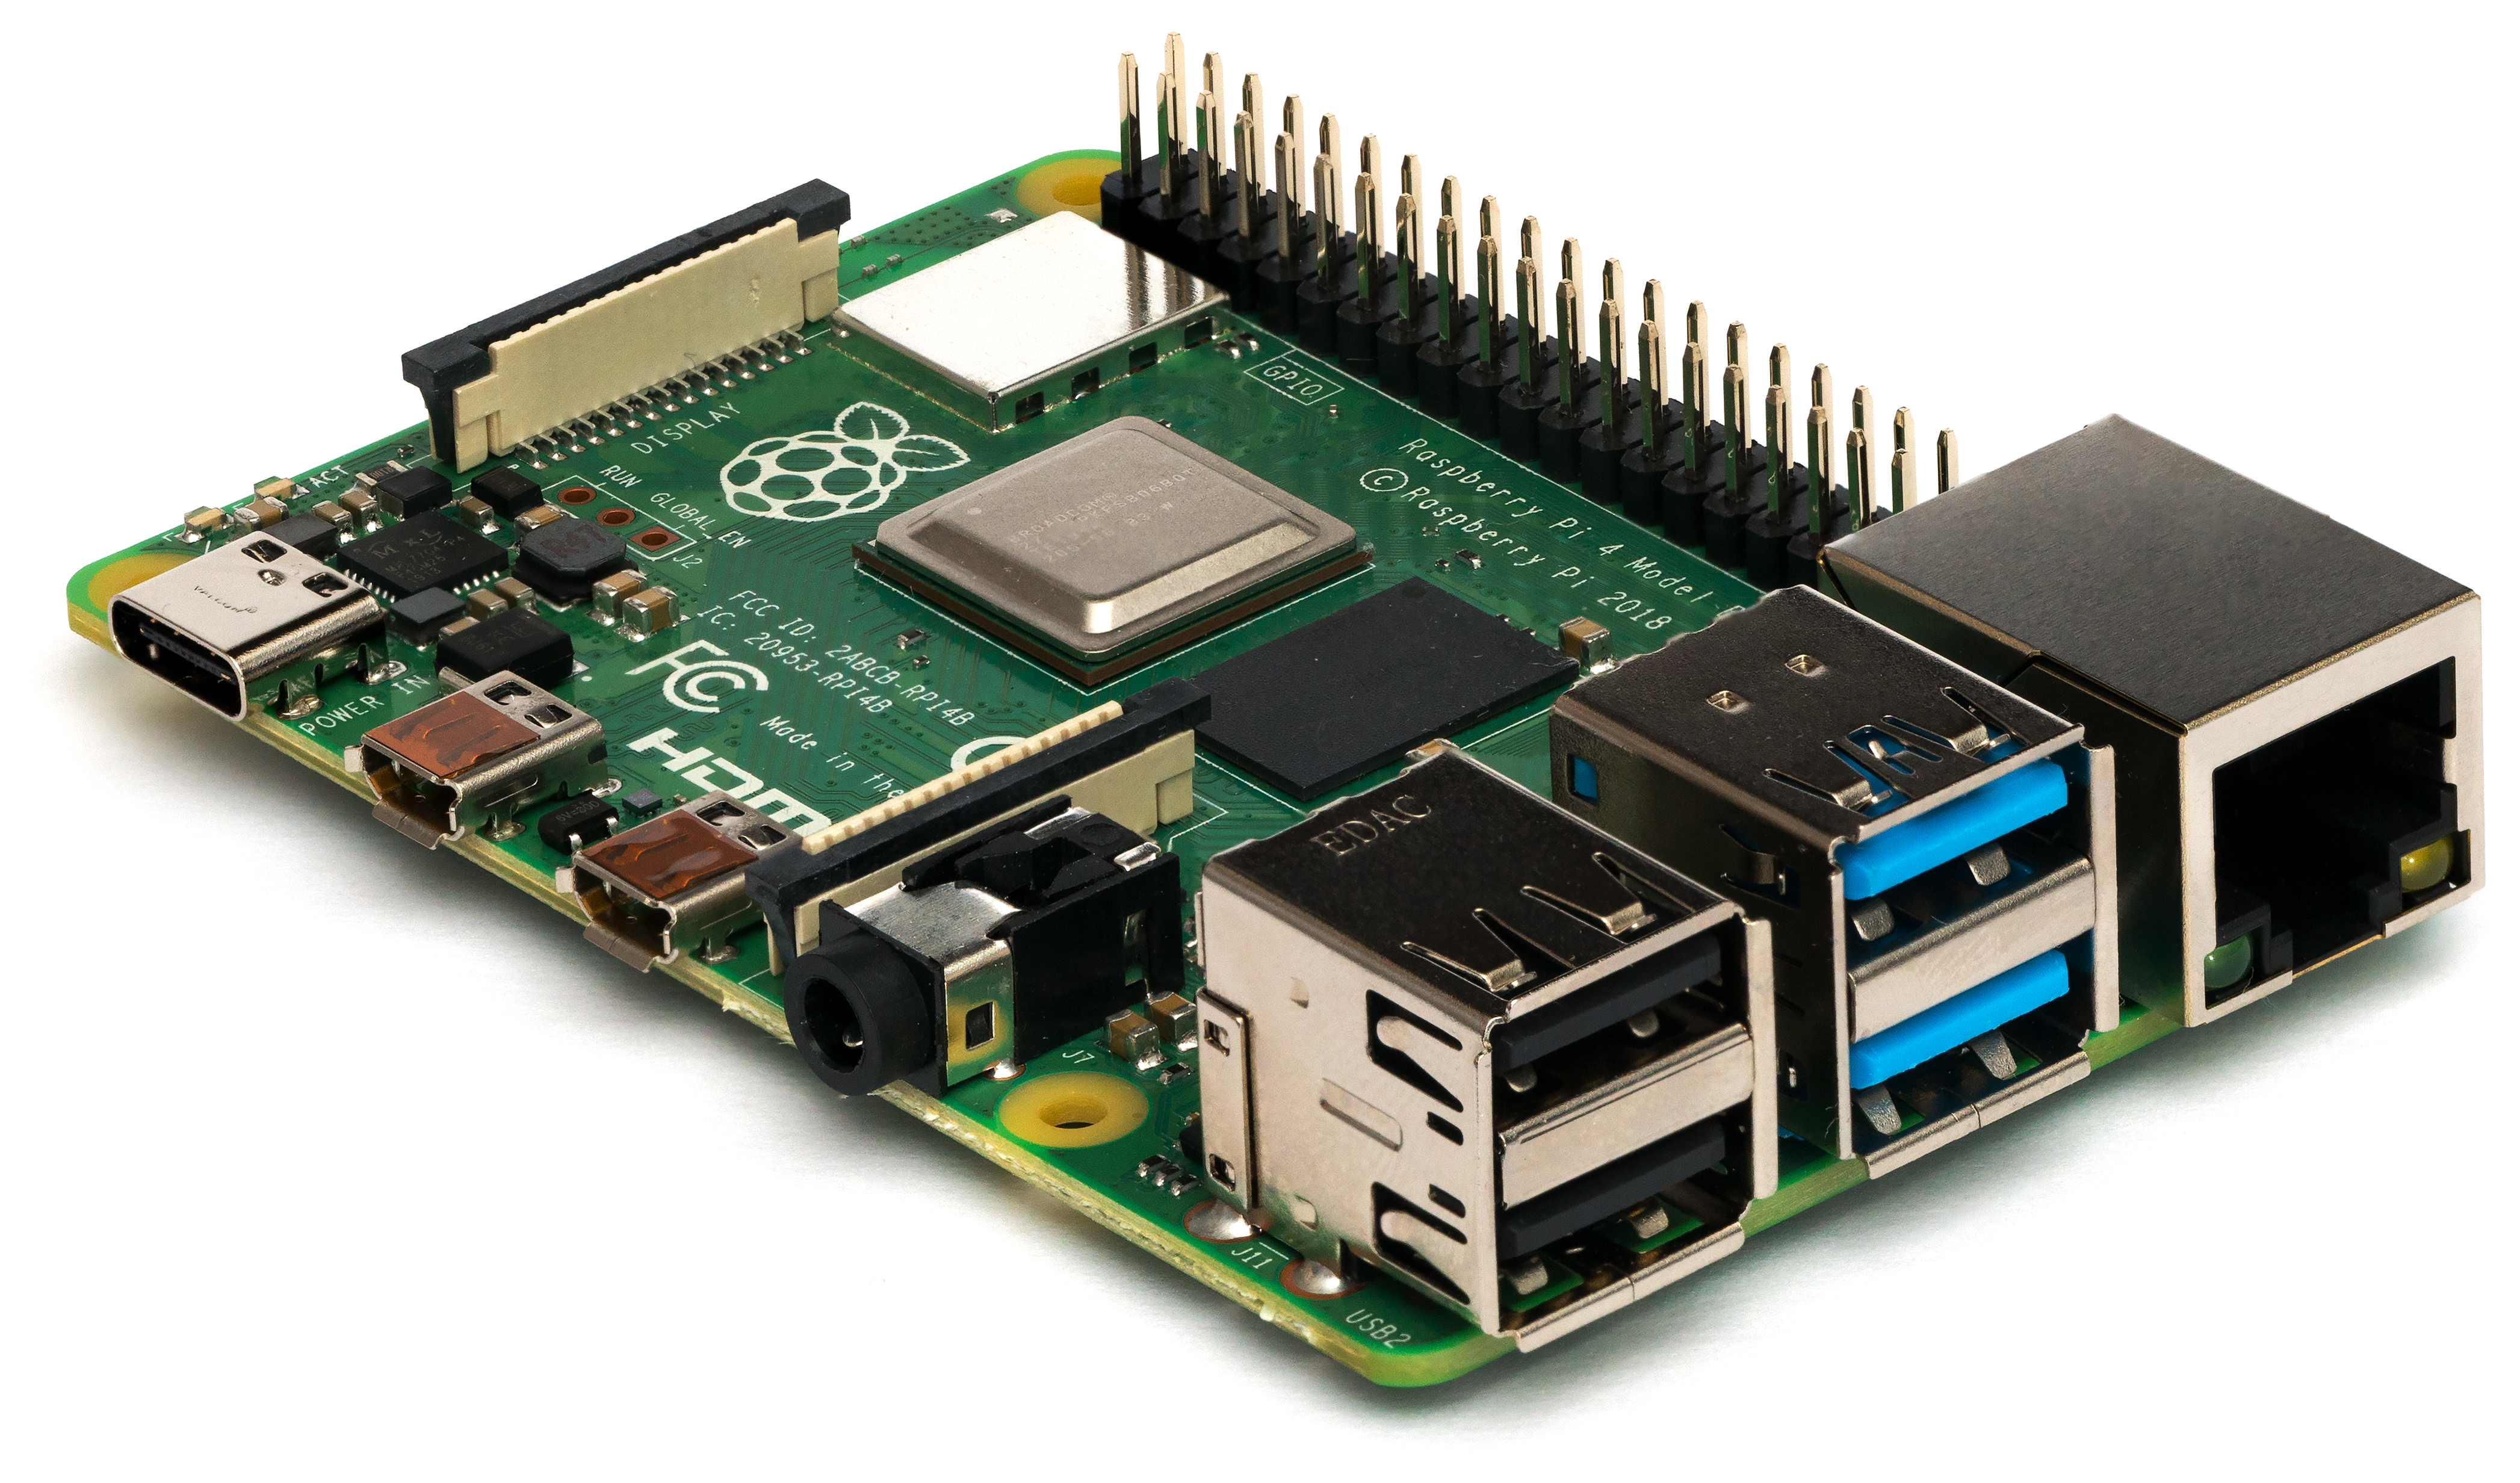
\includegraphics[scale=0.05]{./Figuras/rpi4.jpg}
\caption{Raspberry Pi 4 modelo B}
\label{fig:rpi4}
\vspace*{-10pt}
\end{figure}

\item Raspberry Pi 400: Cuenta con una placa personalizada que se deriva de la Raspberry Pi 4 existente, específicamente remodelada para incluirla en un teclado derivado del Raspberry Pi Keyboard. Posee una solución de enfriamiento mas robusta que su contraparte 4 modelo B al poseer una placa de metal ancha para disipar el calor y un conmutador actualizad para la fuente de alimentación que es un poco mas alta que la del Raspberry Pi 4. La computadora cuenta con 4GB de memoria RAM LPDDR4.
\item Raspberry Pi Pico: Anunciada en el 2021, es una placa pequeña y versátil construida con RP2040, un nuevo chip microcontrolador diseñado por Raspberry Pi Fundation. Este modelo está gobernada por un pequeño SoC que cuenta con un procesador dual core ARM Cortex M0+ funcionando a 133 MHz, acompañado de 264 KB de RAM y 2 MB de almacenamiento integrado.
\item Raspberry Pi 5: La mas nueva de las versiones del Raspberry Pi existentes al momento de la escritura de esta investigación representa el salto de rendimiento sobre el modelo anterior de Raspberry Pi 4. Con un procesador  Broadcom BCM2712 casi duplica la frecuencia del CPU con respecto a su predecesora, además de contar ahora con una nueva GPU VideoCore VII mucho más rápida con una frecuencia de 800 MHz. Entre otras mejoras.
\end{itemize}
Existen gran variedad de sistemas operativos que pueden ser usados con este micro computador, la mayoría de ellos, basados en Linux, pero también con la posibilidad de instalar Windows 10 (Iot Core) o Android (Android Things).\\

Una característica principal de estas placas es la existencia de 40 pines GPIO, los cuales proveen entradas y salidas digitales para el micro computador con lo que se le puede expandir su s funcionalidades con el uso de sensores (HATs o a través de circuitos eléctricos tradicionales), cuya lógica puede ser creada en lenguajes de programación como Python, C++, Java, entre otros.\\

El proyecto ha ganado una comunidad muy amplia alrededor del mundo, que han probado la versatilidad que posee este micro computador en proyectos de toda índole, dando a las personas la capacidad de crear soluciones basadas en IoT con una relación coste-rendimiento positivo.


%	capitulo cinco
%-----------------------------------------------------------------------------
%	 Marco Aplicativo
%-----------------------------------------------------------------------------

\lhead[\thepage]{Metodología General de Trabajo \thechapter. \rightmark}
\rhead[Metodología General de Trabajo \leftmark]{\thepage}
\part{Marco Aplicativo}
%	Capitulo 6: Metodología General de Trabajo
\chapter{Metodología General de Trabajo}
\markboth{Metodología General de Trabajo}{Metodología General de Trabajo}

\section{Scrum}
\lhead[\thepage]{\thesection. Scrum}
Scrum es una metodología ágil y flexible para gestionar el desarrollo de software. Se basa en construir primero la funcionalidad de mayor valor para el cliente y en los principios de inspección continua, adaptación, auto-gestión e innovación.\cite{scrumsofteng} En Scrum se aplican de manera regular un conjunto de buenas prácticas para trabajar colaborativamente y obtener el mejor resultado posible de un proyecto.\\

Es parte de la filosofía de Scrum el poder realizar entregas parciales y regulares del producto final, priorizadas por el beneficio que aportan al receptor del proyecto. Por ello, Scrum está especialmente indicado para proyectos en entornos complejos, donde se necesita obtener resultados rápidamente, con requisitos son cambiantes o poco definidos, donde la innovación, la competitividad, la flexibilidad y la productividad son fundamentales.\\

En Scrum un proyecto se ejecuta en bloques temporales cortos y fijos (iteraciones que normalmente son de 2 semanas, aunque en algunos equipos son de 3 y hasta 4 semanas, límite máximo de feedback y reflexión). Cada iteración tiene que proporcionar un resultado completo, un incremento de producto final que sea susceptible de ser entregado con el mínimo esfuerzo al cliente cuando lo solicite. El proceso parte de la lista de objetivos/requisitos priorizada del producto, que actúa como plan del proyecto. En esta lista el cliente prioriza los objetivos balanceando el valor que le aportan respecto a su coste y quedan repartidos en iteraciones y entregas.\\  

La actividades que se llevan a cabo bajo la metodología de Scrum son las siguientes:

\begin{enumerate}
\item Planificación de la iteración: En el primer día de cada iteración, el equipo realza una reunión de planificación de la iteración. Esta etapa consiste en una primera fase de selección de requisitos, en la cual el cliente presenta al equipo la lista de requisitos priorizada del proyecto y se responden a las dudas que surgen sobre el dominio de las tareas a realizar y una segunda fase de planificación de la iteración, donde el equipo elabora la listas de tareas necesarias para desarrollar lo que se es requerido para la iteración, ademas de la estimación de esfuerzos por parte de los miembros del equipo.
\item Ejecución de la iteración: Cada día se realiza una reunión con todo el equipo de 15 minutos como máximo para inspeccionar el avance en la realización de las tareas, dependencias u actividades bloqueantes ye insumos pendientes para su culminación. Durante la iteración el Scrum Master (facilitador) se encarga de que el equipo pueda articularse y cumplir los compromisos adquiridos por el equipo.
\item Inspección y adaptación: El ultimo día de la iteración se realiza la reunión de revisión de la iteración. Esta se conforma de dos partes, la demostración en donde el equipo presenta al cliente el/los entregable(s) con los requisitos mínimos acordados y la retrospectiva en la que el equipo analiza si su manera de trabajar ha sido la adecuada, los problemas que han surgido, su solución, de forma que se pueda mejorar de manera continua la productividad.
\end{enumerate}

\section{Control de Versiones de Software}
\lhead[\thepage]{\thesection. Control de Versiones de Software}
Un software de control de versiones es un aquel que permite registrar y gestionar cambios a nivel del código fuente de manera histórica permitiendo retornar a versiones anteriores o comprar diferencias entre ellas.

Esto permite tener:
\begin{itemize}
\item Flujos de trabajo organizados:
\item Descripción de versiones:
\item Colaboración:
\item Historial de cambios: 
\end{itemize}

\subsection{Git}
Git es un sistema de control de versiones moderno, distribuido y seguro que fue desarrollado originalmente por Linus Torvalds en el año 2005. 

Entre sus características principales se destacan:
\begin{itemize}
\item Arquitectura distribuida:
\item Flexibilidad:
\item Seguridad:
\item Rendimiento:
\end{itemize}

\subsubsection{Git-Flow}
Git Flow es una metodología para usar Git en la que se combina ramas de función y ramas principales. Fue popularizado por Vincent Driessen en 2010. Los aspectos clave del modelo Git Flow son:
\begin{itemize}
\item Ramas principales y de desarrollo: En lugar de tener una única rama principal, Git Flow utiliza dos ramas principales:
\begin{enumerate}
\item Main (o Master): Almacena el historial oficial de publicación.
\item Develop: Sirve como rama de integración para las funciones.
\end{enumerate}
\item Ramas de función: Los desarrolladores crean ramas de función para trabajar en características específicas. Estas ramas se fusionan con develop cuando la función está completa.
\item Ramas de publicación y corrección de errores:
\begin{enumerate}
\item Release Branches: Se crean a partir de develop para preparar una nueva versión. Aquí se realizan pruebas finales y se corrigen errores antes de la publicación.
\item Hotfix Branches: Se utilizan para corregir errores críticos en la versión actual de producción. Se crean a partir de main y se fusionan tanto con main como con develop.
\item Versionado y etiquetado: Git Flow simplifica la gestión de versiones al asignar números de versión a las confirmaciones en main y etiquetarlas.
\end{enumerate}
\end{itemize}

\section{Herramientas de Desarrollo}
\lhead[\thepage]{\thesection. Herramientas de Desarrollo}
A continuación se detalla aquellas herramientas de hardware y de software utiizados durante el desarrollo de este trabajo de investigación.

\subsection{Herramientas de Hardware}
Dado el enfoque de tener un grupo de dispositivos IoT que pudiesen obtener data real del entorno en donde fuesen desplegados, se obtuvo un conjunto de placas programables, microcomputadores y microcontroladores, así como también de sensores y actuadores para poder crear prototipos funcionales. Se contó con cuatro placas programables de distinta índole:
\begin{itemize}
\item Dos Raspberry Pi modelos 3 B.
\item Un Raspberry Pi Zero.
\item Un Arduino Uno R3.
\end{itemize}

Entre los sensores y actuadores a integrar a esos dispositivos se ha contado con los siguientes elementos:
\begin{itemize}
\item Dos sensores de movimiento PIR HC-SR501.
\item Un sensor de test de nivel de agua Robodo Sen18.
\item Un sensor de temperatura DS1820.
\item Dos leds RGB.
\item Una fotorresistencia (LDR).
\item Un sensor de temperatura y humedad DHT11.
\item Dos leds color verde.
\item Dos leds color rojo.
\item Seis leds color blanco.
\item Un sensor de intensidad lumínica TSL2561.
\item Un buzzer HW-508.
\item Una pantalla LCD 16x2 I2C Hd44780.
\item Un Lector de tarjetas RFID RC522.
\item Un llavero RFID 100.
\item Una tarjeta RFID programable. 
\item Una cámara RaspiCam V1.  
\end{itemize}

Por otro lado para el desarrollo de software se hizo uso de un computador con las siguientes características:
\begin{itemize}
\item CPU
\item RAM
\item Almacenamiento
\item Sistema Operativo
\end{itemize}

Finalmente el software desarrollado fue desplegado en uno de los dispositivos Raspberry Pi 3 modelo B cuyas características son:
\begin{itemize}
\item CPU
\item RAM
\item Almacenamiento
\item Sistema Operativo
\end{itemize}

\subsection{Python}
Python es un lenguaje de programación de alto nivel, multiplaforma,  débilmente tipado de propósito general, multiparadigma e interpretado\cite{whatspython}, creado por Guido Van Rossum. Su filosofía se basa en el poder crear código que sea muy legible, con una sintaxis simple, utilizando indentaciones para delimitar bloques de código, mas corto y potente que en otros lenguajes de programación.\cite{Guido}\\

Se dice que Python es un lenguaje que viene con "pilas puestas"\cite{pep206}, es decir, que de por si, posee un conjunto de funciones amplio para afrontar cualquier tipo de situación dentro de las librería estándar del lenguaje y destaca en su facilidad para aprender y alta portabilidad y es usado en un una gran cantidad de aplicaciones, que van desde el área web, pasando por la ciencia de datos, la inteligencia artificial y la programación de dispositivos.  

\begin{figure}[ht]
\centering
\includegraphics[width=0.4\textwidth]{Figuras/python-logo.png}
\caption{\label{fig:python-logo}Logo de Python}
\vspace*{-10pt}
\end{figure}

\subsection{Django}
Django es un framework web de alto nivel que permite el desarrollo rápido de sitios web seguros y mantenibles. Desarrollado por programadores experimentados, Django se encarga de gran parte de las complicaciones del desarrollo web, por lo que puedes concentrarte en escribir tu aplicación sin necesidad de reinventar la rueda. Es gratuito y de código abierto

\subsection{Bases de datos}
Para el desarrollo de la aplicación web se desplegaron dos bases de datos para poder aprovechar las caracteristicas de los datos y flujos involucrados:
\begin{itemize}
\item Una base de datos Postgresql para la gestión de los datos y elementos de la aplicación web en si misma.
\item Una base de datos InfluxDB para almacenamiento de la información registrada por la operación de los sensores y actuadores de los dispositvos IoT.
\end{itemize}

\subsubsection{Postgresql}
Es un sistema de gestión de bases de datos relacional orientado a objetos y de código abierto. Sus principales caracteristicas son:
\begin{itemize}
\item Alta concurrencia.
\item Amplia cantidad de tipos nativos.
\end{itemize}

\subsubsection{InfluxDB}
Es una base de datos de series temporales de código abierto desarrollada por InfluxData, utilizada para almacenar y recuperar datos de series temporales en áreas como monitoreo de operaciones, métricas de aplicaciones, datos de sensores de Internet de las Cosas y análisis en tiempo real. Está escrita en el lenguaje de programación Rust.

\subsection{Eclipse Mosquitto}
Eclipse Mosquitto es un broker de mensajes de código abierto que implementa las versiones 5.0, 3.1.1 y 3.1 del protocolo MQTT. Es ligero y adecuado para todos los dispositivos, desde computadoras de placa única de baja potencia hasta servidores completos. Esta escrito en el lenguaje de programación C.

\subsection{Grafana}
Grafana es una plataforma de visualización de código abierto que permite generar métricas, registros y trazas de datos de otras aplicaciones a través del uso de graficos y tablas organizados en dashboards. Permite consultar, visualizar, configurar alertas y comprender tus métricas, sin importar dónde se almacenen. 

\subsection{Node-Red}
Node-RED es una herramienta de programación que te permite conectar, integrar y automatizar dispositivos de hardware, APIs y servicios en línea. Su editor basado en paneles dentro del navegador facilita la creación de flujos mediante una amplia variedad de nodos, que luego se pueden implementar en su entorno de ejecución al mismo tiempo de manera sencilla.

\subsection{Docker}
Docker es una plataforma de código abierto que simplifica y automatiza el proceso de construir, desplegar y gestionar contenedores. Los contenedores son componentes estandarizados y ejecutables que combinan el código de la aplicación con las dependencias del sistema operativo.

\section{Adaptación del Marco Metodológico}
Para llevar a cabo la investigación propuesta, se decidió adaptar la metodología de forma que está favoreciera el desarrollo de los diversos elementos que se requerían. De esta manera se acordó hacer uso de lo siguiente:
\begin{itemize}
\item Sprints de dos semanas de duración.
\item Reuniones mensuales para realizar retrospectiva, sprint review y planificación de actividades para los siguientes sprints. Reunión en formato daily cada semana para comentar avances, bloqueos y recursos requeridos.  
\item Hacer entregas incrementales basadas en la adición de features y correcciones de código cada final de sprint.
\item Kick off del proyecto para el mes de septiembre del 2018.
\item Duración estimada del desarrollo de los dispositivos y de la aplicación web de 9 sprints (18 semanas).
\item El profesor Antonio Russoniello en calidad de tutor del trabajo especial de grado, asume el rol de Scrum Master. 
\item El bachiller Pedro Boll asume el desarrollo. 
\end{itemize}
Con ello definido, se presentan las siguientes actividades para el desarrollo y culminación del proyecto según los objetivos generales y especificos en la  tabla \ref{tabla:actividades_desarrollo}, junto con su duración aproximada.

\begin{table}[!htb]
\centering
\begin{tabular}{| m{4.5cm}| m{6.6cm}| m{3.2cm}|}
\hline
\multicolumn{3}{|c|}{Actividades de desarrollo} \\
\hline 
\centering Actividad & \centering Descripción & \centering Tiempo Estimado \tabularnewline \hline
1 & 2 & 3 \\ \hline
\end{tabular}
\caption{Actividades sugeridas para el desarrollo del trabajo especial de grado}
\label{tabla:actividades_desarrollo}
\end{table}
 
%	Capitulo seis
%-----------------------------------------------------------------------------
%	 Diseño e Implementación
%-----------------------------------------------------------------------------

\lhead[\thepage]{Diseño e Implementación \thechapter. \rightmark}
\rhead[Diseño e Implementación \thechapter.1 \leftmark]{\thepage}

%	Capitulo 6: Diseño e Implementación
\chapter{Diseño e Implementación}
\markboth{Diseño e Implementación}{Diseño e Implementación}

%	Sección uno: Diseño de la solución
\section{Diseño de la solución}
\lhead[\thepage]{\thesection. Diseño de la solución}

\begin{figure}[htb]
\centering
\includegraphics[scale=0.4]{./Figuras/rpi3javier.png}
\caption{huehuehuehuhehuehuehue}
\label{fig:hue}
\vspace*{-10pt}
\end{figure}

%	Sección dos: Implementación  de la solución 
\section{Implementación de la solución}
\lhead[\thepage]{\thesection. Diseño de la solución}

% Capitulo siete
%-----------------------------------------------------------------------------
%	 Entorno de Pruebas
%-----------------------------------------------------------------------------

\lhead[\thepage]{ Entorno de Pruebas \thechapter. \rightmark}
\rhead[ Entorno de Pruebas \thechapter. \leftmark]{\thepage}

%	Capitulo N:  Entorno de Pruebas
\chapter{ Entorno de Pruebas}
\markboth{ Entorno de Pruebas}{ Entorno de Pruebas}
\section{Escenarios de pruebas}
hue

\subsection{Dispositivos IoT}
hue
\subsubsection{Raspberry Pi 3B}
hue
\subsubsection{Raspberry Pi Zero}
hue
\subsubsection{Arduino Uno}
hue

\subsection{Aplicación HAMACA}
hue
\subsubsection{Captura de Información}
hue
\subsubsection{Visualización de datos}
hue
\subsubsection{Monitoreo de Dispositivos}
hue
\subsubsection{Control de Dispositivos}
hue
%	Capitulo ocho
%-----------------------------------------------------------------------------
%	 Casos de Uso 
%-----------------------------------------------------------------------------

\lhead[\thepage]{Casos de Uso \thechapter. \rightmark}
\rhead[Casos de Uso \thechapter. \leftmark]{\thepage}

%	Capitulo 8: Casos de Uso
\chapter{Casos de Uso}
\markboth{Casos de Uso}{Casos de Uso}

\section{Infraestructura de Comunicación}
\lhead[\thepage]{\thesection. Infraestructura de Comunicación}
En la solución prevista, específicamente hablando de los componentes que requieren comunicarse usando MQTT como protocolo y el broker, es decir, los dispositivos IoT y la apliación web HAMACA se establece lo siguiente:

\begin{figure}[htb]
\vspace*{-10pt}
\centering
\includegraphics[scale=0.65]{./Figuras/caso_de_uso_mqtt.png}
\caption{Diagrama de caso de uso para la comunicación vía MQTT}
\label{fig:caso_de_uso_mqtt}
\end{figure}

El detalle de cada caso es el siguiente:
\begin{itemize}
\item Conectar dispositivo: Este caso de uso hace referencia a negociar la conexión entre un dispositivo y el broker MQTT utilizado, en este caso, bajo la implementación Mosquitto. Para poder conectarse solo se necesita la dirección del servicio, se encuentre o no de manera local en la red. Ambos actores pueden realizar esta acción.
\item Publicar Tópico: Para poder comenzar a comunicarse, se tiene que definir un tópico para que pueda ser escuchado/leído por cualquier dispositivo con acceso. 
\item Crear mensaje: Simplemente se envia un mensaje MQTT con el tópico definido y el contenido útil de dicho mensaje
\item Consumir mensaje: MQTT sigue le paradigma de publicación, suscripción por lo que es posible que cualquiera que este suscrito a un tópico será capaz de leer el mensaje y este no estará más disponible. 
\end{itemize}

\section{Aplicación Web}
\lhead[\thepage]{\thesection. Aplicación Web}
Para el caso de la aplicación web HAMACA, se consideraron dos tipos de usuarios que interectuaran con ella. El primer es un usuario administrador que tiene privilegios por sobre todas las acciones disponibles y un usuario final cualquiera que solo podrá gestionar las acciones que tengan que ver con la visualización, monitoreo y control de dispositivos IoT, sus sensores, actuadores y la data asociada a ellos como se puede ver en el diagrama de la figura \ref{fig:caso_de_uso}\\

\begin{figure}[!htb]
\vspace*{10pt}
\centering
\includegraphics[scale=0.45]{./Figuras/caso_de_uso.png}
\caption{Diagrama de caso de uso para la aplicación web HAMACA}
\label{fig:caso_de_uso}
\vspace*{-5pt}
\end{figure}

A continuación se explica cada acción dentro del caso de uso:

\begin{itemize}
\item Gestionar usuario: Se refiere a la capacidad de administrar los aspectos concernientes a los usuarios de la aplicación. Solo puede ser accedido por los usuarios administradores.
\item Crear usuario: Consiste en llenar el formulario con la información del usuario nuevo de la plataforma para ser guardado en base de datos.
\item Editar usuario: Consiste en editar la información existente de un usuario en particular en cualquiera de los elementos disponibles. Se puede editar el nombre, apellido, correo electrónico o la contraseña. Lo realiza el usuario administrador.
\item Eliminar usuario: Se borra de la aplicación un usuario. Solo puede borrar el usuario administrador.
\item Configurar fuente de datos: Para la configuración inicial de Grafana es requerido crear una conexión a una fuente de datos. Esta acción es para solo aquellos que tiene el rol de admin del sistema.
\item Controlar dispositivo: Se refiere a poder usar la interfaz de control para poder realizar una o mas acciones de control sobre uno o más dispositivos IoT Esto lo puede hacer cualquier usuario.
\item Gestionar cuadro de mando: Esta es la acción de administrar lo concerniente a los dashboards o cuadros de mando que posee la integración de Grafana. Puede ser realizado por cualquier usuario.
\item Crear cuadro de mando: Representa la acción de poder crear un nuevo cuadro de mando desde cero. Puede ser realizado por cualquier rol de usuario.
\item Modificar cuadro de mando: Está acción conlleva editar cualquier cuadro de mando que ya haya sido creado. Puede ser realizado por cualquier usuario.
\item Eliminar cuadro de mando: Esta acción simplemente borra un cuadro de mando de la integración. Puede realizarla cualquier usuario.
\item Crear indicador: Esta acción consiste en crear un indicador (gráfico, texto, alerta, etc) sobre un cuadro de mando. Debe existir un cuadro de mando al menos para ello y esta acción puede ser llevada a cabo por cualquier rol de usuario.
\item Editar indicador: Esta acción consiste en editar un indicador existente en un cuadro de mando. Puede ser realizada por cualquier usuario. 
\item Eliminar indicador: Consiste en borrar un indicado sobre un cuadro de mando. Puede ser llevada a cabo por cualquier usuario.
\item Gestionar flujo de automatización: Se refiere a la capacidad de administrar uno o mas flujos de automatización de la aplicación haciendo uso de la integración de la herramienta Node-Red. Esta acción puede ser llevada a cabo por cualquier tipo de usuario.
\item Crear flujo de automatización: Esto es el poder crear un flujo nuevo desde cero para automatizar una o más tareas. Puede ser realizada por cualquier usuario.
\item Desplegar flujo de automatización: Consiste en tomar un flujo de trabajo existe y activarlo para su funcionamiento. Esta acción la puede hacer cualquier usuario.
\item Modificar flujo de automatización: Como su nombre lo dice, se refiere a la capacidad de los usuarios de editar un flujo de trabajo existente, sin importar que rol posean. 
\item Eliminar flujo de automatización: Cualquier usuario tiene la potestad de poder borrar un flujo de trabajo existe.
\item Crear tarea: Esto es la capacidad de crear una tarea para automatizar sobre uno o mas sensores/actuadores de uno o más dispositivos. Se requiere que exista un flujo de trabajo sobre el cual hacer esto. Es una acción que puede realizar cualquier usuario.
\item Editar tarea: Significa que se cambien características o instrucciones sobre una  tarea existente. Esta acción la puede realizar cualquier usuario.
\item Eliminar Tarea: Hace referencia a la capacidad de borrar una tarea existente sobre un flujo de trabajo. Esto es posible para cualquier usuario, independientemente de su rol.
\end{itemize}
%	Capitulo nueve
%-----------------------------------------------------------------------------
%	 Resultados, Limitaciones y Trabajos Futuros
%-----------------------------------------------------------------------------

\lhead[\thepage]{Resultados, Limitaciones y Trabajos Futuros \thechapter. \rightmark}
\rhead[Resultados, Limitaciones y Trabajos Futuros \thechapter. \leftmark]{\thepage}

%	Capitulo N: Conclusiones
\chapter{Resultados, Limitaciones y Trabajos Futuros}
\markboth{Resultados, Limitaciones y Trabajos Futuros}{Resultados, Limitaciones y Trabajos Futuros}
hue
\section{Resultados}
hue
\section{Limitaciones}
hue
\section{Contribuciones}
hue
\section{Trabajos Futuros}
hue
%	Capitulo diez
%-----------------------------------------------------------------------------
%	 Conclusiones
%-----------------------------------------------------------------------------

\lhead[\thepage]{Conclusiones \thechapter. \rightmark}
\rhead[Conclusiones \thechapter. \leftmark]{\thepage}

%	Capitulo N: Conclusiones
\chapter{Conclusiones}
\markboth{Conclusiones}{Conclusiones}

Este trabajo de investigación permitió demostrar la factibilidad del desarrollo de una herramienta de visualización de datos, monitoreo, control y automatización de procesos concernientes a dispositivos de internet de las cosas, partiendo desde prototipos funcionales que pudiesen generar información para llevarlo a un escenario lo más realista posible sobre el como de desplegaría un futuro contexto donde los artefactos inteligentes son ubicuos.\\

El desarrollo de prototipos de dispositivos IoT permitió identificar las fortalezas y debilidades de los enfoques utilizados para medir y controlar estos artefactos de manera transparente. Se observaron como el fenómeno de la variedad entre sensores, actuadores y dispositivos en si pueden generar data que aunque representen lo mismo tiene matices de eficiencia y eficacia que pueden ser aprovechados por otros elementos en la búsqueda de capturar, mostrar y utilizar la información que capturamos de ellos.\\

Por el lado del desarrollo de la aplicación web se demostró que un software que pueda orquestar e integrar herramientas existentes para tareas especificas como visualización de datos, automatización de procesos, monitoreo y control de dispositivos puede ser una alternativa viable para poder centralizar las operaciones inherentes a dispositivos IoT y que es un esquema flexible que permite no solo adaptarse a las necesidades de los usuarios sino también con alta capacidad de crecimiento futuro, sea desde el punto de vista de protocolos y estándares, como de software análisis automatizado.\\

Finalmente, se considera que los objetivos planteados en el marco del planteamiento del problema fueron cumplidos con éxito y se espera que este software sea al final de utilidad en donde el contexto permita aprovechar las funcionalidades desarrolladas anteriormente, sea dentro del ámbito académico, investigativo, industrial o uso personal.


%	Referencias bibliográfica
\lhead[\thepage]{BIBLIOGRAFÍA}
\bibliography{Referencias/Referencias}
\end{document}
